\documentclass{article}

\usepackage[margin=0.75in]{geometry}
\usepackage{amsmath,amssymb}
\usepackage{graphicx,float}
\usepackage{multirow,setspace}
\usepackage{natbib,enumerate}
\usepackage{caption}
\usepackage{subcaption}
\usepackage{termcal} 
\usepackage{xcolor}
\usepackage{enumitem}
\usepackage{gensymb}
\usepackage{multicol}
\usepackage{listings}
\usepackage{booktabs}


\setlength{\marginparwidth}{2cm}

\renewcommand{\thesection}{\Alph{section}}
\newcommand{\HRule}{\rule{\linewidth}{0.5mm}}
\newcommand{\tab}{\hspace{0.5cm}}
\newcommand{\modref}[1]{(\ref{#1})}

\newcommand{\bbeta}{{\mbox{\boldmath$\beta$}}}
\newcommand{\bmu}{{\mbox{\boldmath$\mu$}}}
\newcommand{\balpha}{{\mbox{\boldmath$\alpha$}}}
\newcommand{\btheta}{{\mbox{\boldmath$\theta$}}}
\newcommand{\bpi}{{\mbox{\boldmath$\pi$}}}
\newcommand{\R}{\texttt{R}}
\newcommand{\Lik}{\mathcal{L}}

\begin{document}

%%% HEADER %%%
	\begin{center}
		\HRule \\[0.1cm]
		\vspace{0.1cm}
		{ \LARGE \bfseries MATH 2625: Biostatistical Methods\\[0.5cm] Homework 4, due Thursday, March 27 } \\[0.1cm]
		\HRule \\[0.1cm]
	\end{center}
	
		Please submit a PDF or .doc version of your homework to Canvas by 3:30pm on the due date. Please type \emph{all} responses. You are encouraged to use \R\ for all calculations.

		Fritze Mayer \& Yu Fan Mei
		
	\section*{Theory}
	\begin{enumerate}
		\item For the Mantel-Haenszel odds ratio estimator applied to matched proportions, $\tilde{\theta} = \frac{n_{21}}{n_{12}}$, an estimate of the uncertainty can be constructed by noting that the variance of the $\log(\tilde{\theta})$ is
		\begin{align*}
			\widehat{Var}\left[\log(\tilde{\theta})\right] = \frac{1}{n_{21}} + \frac{1}{n_{12}}.
		\end{align*}
		Using this, construct an $\alpha$-level confidence interval for $\tilde{\theta}$. State any relevant assumptions.
	\end{enumerate}

	For the matched proportions odds ratio 

	\section*{Case Studies}
	For each of the following case studies, create a structured abstract no longer than 4 pages in length (including figures, tables, and references). The Background section is provided for each and should be included in your write-up. You must write the Methods, Results, and Conclusion sections. Code should be included in an appendix as well.

	\begin{enumerate}
		\item Consider a study that examined maternal stress in utero to subsequent childhood wheezing. The data is in the file \texttt{whz.txt} alongside this assignment. The variable \texttt{wheeze} is coded 1 if the child had repeated wheezing events, 0 if the child did not. The variable \texttt{stress} is coded 1 if the mother had elevated bed time stress and 0 if she did not. The variables \texttt{sex} (1 for female, 0 for male), \texttt{smoker} (1 if the mother smoked during pregnancy, 0 if she did not), and \texttt{atopy} (1 for yes, 0 for no) contain the possible confounders. Adjustments for each possible confounder should be performed separately.
	
	\subsubsection*{Data Structure in \R}
	
	You will need to put the data into $2\times2\times K$ arrays. To do this, we can use the \texttt{table()} command where the first entry is the $X$, the second entry is the $Y$, and the third entry is the $Z$. For example, a properly formatted table with \texttt{sex} as $Z$ can be generated using
	\begin{lstlisting}[language = R]
with(whz, table(stress, wheeze, sex))
	\end{lstlisting}

	
	\item In this case study, you will examine the agreement between primary care physicians and psychiatrists, termed specialty care for this analysis, on a set of five indicators. Each indicator denotes whether primary care or specialty care made contact with agency within a system of care framework for managing pediatric mental health. The data is in the file \texttt{soc.txt} alongside this assignment. The variables \texttt{eduPC}, \texttt{cpsPC}, and \texttt{mhPC} denote whether or not primary care (PC) made contact with the respective agency. The variables \texttt{eduSC}, \texttt{cpsSC}, and \texttt{mhSC} denote whether or not specialty care (SC) made contact with the respective agency.

	\subsubsection*{Data Structure in \R}
	
	The data is structured in the \emph{wide} format where each row corresponds to one subject and columns can correspond to multiple measurements. This structure is useful for making population-averaged tables. Thus to get the population averaged table for one of the agencies, say mental health, we could use the following:
	\begin{lstlisting}[language = R]
with(soc, table(mhPC, mhSC))
	\end{lstlisting}

	\end{enumerate}

	

	\newpage
	\subsection*{Background}
	
	Early childhood wheezing, defined as more than one wheezing event in the first three years of life, can be a precursor to the development of asthma. Early identification of children who may potentially develop asthma could lead to early interventions that mitigate the effects. A study was conducted among an urban Boston cohort of 258 pregnant women. On a single day during the second trimester of pregnancy, each woman collected sputum swabs at five times throughout the day: when she first woke up, two hours after waking up, six hours after waking up, two hours before bed, and right before bed. The level of cortisol, a hormone that can be used to measure stress, was measured from each of these samples. Multiple samples were needed as cortisol level naturally vary through out the day. The mothers were then followed through pregnancy and up through the first three years of the child's life to determine the child wheezed or not. Childhood wheezing can be caused by many factors, such as the sex of the child, whether or not the mother smoked during pregnancy, and genetic factors.
	
	Since cortisol levels should naturally be at their lowest right before bed, we are interested in looking for an association between elevated stress levels right before bed and whether or the child experience repeated wheezing in the first three years of life. However, wheezing in children is sex-linked with typically males experience more wheezing events than females. Also, in utero exposure to nicotine may impact lung development. Finally, genetic factors as measured through the phenotype of maternal atopy (i.e. presence of maternal allergies or asthma) may predispose children to wheezing events.

	\subsection*{Methods}
	258 pregnant women were randomly selected from the Boston area for this cohort study. During their pregnancies, we examined their smoking status as well as their mean cortisol levels during the second trimester. We compared their mean cortisol level throughout the day to their cortisol levels right before going to bed. A significant increase in the mothers’ cortisol levels prior to sleeping compared to throughout the day was indicated as an increase in stress. When the children were three years of age, they were examined to see whether or not they developed a wheeze. We also checked to see whether or not the children showed signs of atopy— a genetic predisposition to developing allergic diseases such as asthma, rhinitis, and eczema, among others.

	To control for the potential interaction of the child’s gender on wheezing results, we stratified results based on whether the child was male or female. We calculated the conditional odds ratios before assessing their homogeneity using a Breslow-Day Test. If appropriate, we then used a Mantel-Haenszel Test to determine whether elevated stress levels before sleeping during pregnancy were associated with the child developing a wheeze. We repeated these analyses for the other confounding variables, stratifying for the smoking status of mothers and atopy in the children. All hypothesis tests were conducted at the nominal level in R.

	\subsection*{Results}
	Among the 258 pregnancies, 127 turned out to be male, while the remaining 131 were female. 212 of the mothers smoked, while 46 did not. 164 of the children were not atopic, while 94 of the children showed some form of atopy. Figure 1 shows the presence and absence of maternal elevated bedtime stress, childhood wheezing, sex, maternal smoking status, and child atopy status for all study participants. 

	\begin{table}[h]
		\centering
		\footnotesize
		\caption{Two-Way Tables Comparing Maternal Stress \& Wheezing in Children}
		\begin{minipage}{0.48\linewidth}
			\centering
			\textbf{Male Children} \\[2pt]
			\begin{tabular}{cccc} % Changed to cccc (no vertical bars)
				\toprule
				\textbf{Maternal Stress} & \textbf{No Wheezing} & \textbf{Wheezing} & \textbf{Total} \\
				\midrule
				Yes & 100 & 8 & 108 \\
				No & 13 & 6 & 19 \\
				\midrule
				\textbf{Total} & 113 & 14 & 127 \\
				\bottomrule
			\end{tabular}
		\end{minipage}
		\hfill
		\begin{minipage}{0.48\linewidth}
			\centering
			\textbf{Female Children} \\[2pt]
			\begin{tabular}{cccc} % Changed to cccc (no vertical bars)
				\toprule
				\textbf{Maternal Stress} & \textbf{No Wheezing} & \textbf{Wheezing} & \textbf{Total} \\
				\midrule
				Yes & 107 & 7 & 114 \\
				No & 16 & 1 & 17 \\
				\midrule
				\textbf{Total} & 123 & 8 & 131 \\
				\bottomrule
			\end{tabular}
		\end{minipage}
	\end{table}
	
	
	
	\newpage
	\begin{figure}[h!]
		\centering
		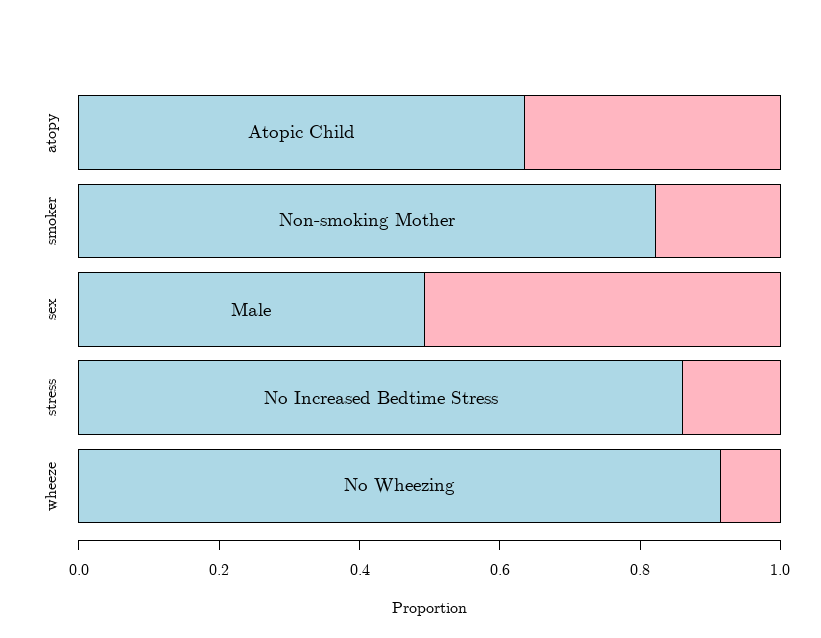
\includegraphics[width=0.6\textwidth]{graphs/stackedBars_case1.png}
		\caption{Proportions of Variables of Interest in Children in the Study \& Their Mothers}
		\label{fig:histogram}
	\end{figure}

	In our study, we found that among male children, the odds of wheezing given mothers showed elevated bedtime stress were 5.77 times greater than if their mothers did not. For female children, the odds of a child wheezing if their mother had elevated bedtime stress were 0.96 times as likely as the odds if their mothers did not have elevated bedtime stress. We found that these odds between sexes were homogenous $(p = 0.134, \chi^2 = 2.243, df = 1)$. After adjustment for sex, we found that the odds of wheezing were significantly higher among children whose mothers had increased bedtime stress during pregnancy than those whose mothers did not show increased bedtime stress during pregnancy ($p = 0.0134$, OR = 3.31, 95\% CI = (1.240, 8.834), CMH $\chi^2 = 6.100)$.


	The odds of wheezing in children whose mothers did not smoke during pregnancy and experienced elevated bedtime stress were 2.78 times greater than in children whose mothers did not experience stress and did not smoke. For children with mothers smoked during pregnancy, the odds of wheezing with mothers who experienced elevated bedtime stress were 10.39 times more than for mothers who did not experience bedtime stress. The Breslow-Day Test confirmed that these odds were homogenous $(p = 0.3395, \chi^2 = 0.9122, df = 1)$. When we adjusted for the confounding influence of maternal smoking, we found that the odds of wheezing were significantly higher among children whose mothers had increased bedtime stress during pregnancy than those whose mothers did not show increased bedtime stress during pregnancy ($p=0.0097$, OR = 3.38, 95\% CI = (1.298, 9.374), CMH $\chi^2 = 6.693)$.

	\begin{table}[h]
		\centering
		\footnotesize
		\caption{Two-Way Tables Comparing Maternal Stress \& Childhood Wheezing, Adjusted for Smoking Status}
		\begin{minipage}{0.48\linewidth}
			\centering
			\textbf{Mother Smoked During Pregnancy} \\[2pt]
			\begin{tabular}{cccc} % No vertical bars
				\toprule
				\textbf{Stress Level} & \textbf{No Wheezing} & \textbf{Wheezing} & \textbf{Total} \\
				\midrule
				No Stress & 171 & 14 & 185 \\
				Stress & 22 & 5 & 27 \\
				\midrule
				\textbf{Total} & 193 & 19 & 212 \\
				\bottomrule
			\end{tabular}
		\end{minipage}
		\hfill
		\begin{minipage}{0.48\linewidth}
			\centering
			\textbf{Mother did not Smoke During Pregnancy} \\[2pt]
			\begin{tabular}{cccc} % No vertical bars
				\toprule
				\textbf{Stress Level} & \textbf{No Wheezing} & \textbf{Wheezing} & \textbf{Total} \\
				\midrule
				No Stress & 36 & 1 & 37 \\
				Stress & 7 & 2 & 9 \\
				\midrule
				\textbf{Total} & 43 & 3 & 46 \\
				\bottomrule
			\end{tabular}
		\end{minipage}
	\end{table}

	\newpage
	\subsection*{Background}

	Many children are treated for mental health disorders in primary care settings.  The system of care (SOC) provides a framework for collaboration among pediatric mental health providers, but it is unclear if youth treated for mental health disorders in primary care receive such coordination.  At the South Boston Community Health Center from 9/2012-8/2013 for 74 individuals $<$18 years, the odds of contact with SOC agencies (the mental health system, the education system, child protective services, the juvenile justice system and developmental disability services) were compared for mental health treatment in primary versus specialty care.  The odds of SOC contact within primary care compared to specialty care specifically for contact with mental health, education and child protective services were examined.  As care coordination may improve health outcomes, increased support and education for care coordination specific to youth treated for mental health disorders in primary care settings may be warranted.
	
	Due to sparsity in two of outcomes (contact with the juvenile justice system and contact with developmental disability services), our study focuses on three agencies: the mental health system (MH), the education system (EDU), and child protective services (CPS). Specifically, we want to examine possible differences between contact with each of the agencies for primary care compared to specialty care. Each subject was seen first by a primary care physician and, later, by a specialty care physician. Specialty care was not made aware of the agencies primary care had recommended contact with. 
	
		
\end{document}














